%!TEX TS-program = xelatex
\documentclass[]{friggeri-cv}
\usepackage{afterpage}
\usepackage{hyperref}
\usepackage{color}
\usepackage{xcolor}
\usepackage{smartdiagram}
\usepackage{fontspec}
% if you want to add fontawesome package
% References:
%   http://texdoc.net/texmf-dist/doc/latex/fontawesome/fontawesome.pdf
%   https://www.ctan.org/tex-archive/fonts/fontawesome?lang=en
%\usepackage{fontawesome}
\usepackage{metalogo}
\usepackage{dtklogos}
\usepackage[utf8]{inputenc}
\usepackage{tikz}
\usetikzlibrary{mindmap,shadows}
\hypersetup{
    pdftitle={},
    pdfauthor={},
    pdfsubject={},
    pdfkeywords={},
    colorlinks=false,           % no lik border color
    allbordercolors=white       % white border color for all
}
\smartdiagramset{
    bubble center node font = \footnotesize,
    bubble node font = \footnotesize,
    % specifies the minimum size of the bubble center node
    bubble center node size = 0.5cm,
    %  specifies the minimum size of the bubbles
    bubble node size = 0.5cm,
    % specifies which is the distance among the bubble center node and the other bubbles
    distance center/other bubbles = 0.3cm,
    % sets the distance from the text to the border of the bubble center node
    distance text center bubble = 0.5cm,
    % set center bubble color
    bubble center node color = pblue,
    % define the list of colors usable in the diagram
    set color list = {lightgray, materialcyan, orange, green, materialorange, materialteal, materialamber, materialindigo, materialgreen, materiallime},
    % sets the opacity at which the bubbles are shown
    bubble fill opacity = 0.6,
    % sets the opacity at which the bubble text is shown
    bubble text opacity = 0.5,
}

\addbibresource{bibliography.bib}
\RequirePackage{xcolor}
\definecolor{pblue}{HTML}{0395DE}

\begin{document}
\header{Nitin}{Prakash}
      {Web developer}
      
% Fake text to add separator      
\fcolorbox{white}{gray}{\parbox{\dimexpr\textwidth-2\fboxsep-2\fboxrule}{%
.....
}}

% In the aside, each new line forces a line break
\begin{aside}
  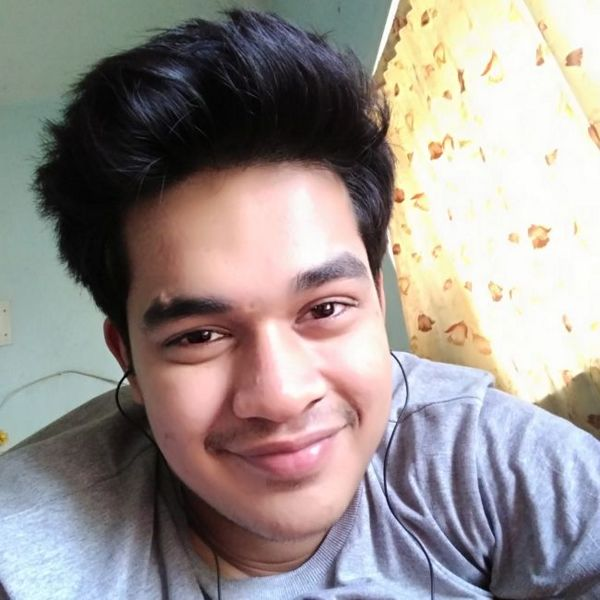
\includegraphics[scale=0.18]{img/dp.jpg}
  \section{Address}
    The LNMIIT
    P.O Sumel, Jamdoli
    Jaipur-302031
    ~
  \section{Tel}
    +91 8769596667
    +91 9905530995
    ~
  \section{Mail}
    \href{mailto: prakash.nitin63@gmail.com}{\textbf{prakash.nitin63@}\\gmail.com}
    ~
  \section{Gitub}
    \href{https://github.com/mygit}{github.com/\\nitinprakash96}
    ~
  % use  \hspace{} or \vspace{} to change bubble size, if needed
  \section{Programming}
    \smartdiagram[bubble diagram]{
        \textbf{C/C++},
        \textbf{Python},
        \textbf{JS},
        \textbf{Linux},
        \textbf{Other\vspace{3mm}},
        \textbf{HTML5}\\\textbf{JQuery},
        \textbf{CSS3},
        \textbf{AngularJS},
        \textbf{Git}
    }
    ~
  \section{Personal Skills}
    \smartdiagram[bubble diagram]{
        \textbf{Team}\\\textbf{Player},
        \textbf{Initiative},
        \textbf{Curiosity},
        \textbf{Problem}\\\textbf{Solving},
        \textbf{\vspace{2mm}Manage\vspace{2mm}},
        \textbf{Organize}
    }
    ~
\end{aside}
~
\section{ Projects}
\begin{entrylist}
  \entry
    {2015}
    {Web design}
    {IEEE}
    {Designed and developed a website for IEEE's event AISYWC. Data validation and animations were done using JavaScript for the most parts and design care was taken by Bootstrap and CSS \\}
  \entry
    {2015}
    {Web Developement}
    {TCO}
    {Developed a gitter room extension at Topcoder's regional event for chrome browser. HTML, CSS, JS and react were the main components of our team. \\}
    \entry
    {2014 - 2015}
    {Part-time collaboration}
    {Freelancer}
    {Has solved some major CSS and PHP bugs in wordpress templates asked by freelancer's clients. \\}
    \entry
    {2015}
    {Webmaster}
    {LNMIIT}
    {Designed and developed LNMIIT's student branch website for IEEE chapter which again used HTML, CSS, Bootstrap, JS and JQuery.}
\end{entrylist}
\\
\section{Education}
\begin{entrylist}
  \entry
    {2005 - 2009}
    {Bachelor's Degree in Computer Sciences}
    {School}
    {Current CPI: 6.00 \\Main Courses: C programming, IT Workshop, Data Structures, Design and Analysis of Algorithms, Theory of Computation, Computer Networks, OOP with Java\\}
  \entry
    {2012 - 2014}
    {Gyan Niketan, India}
    {High School}
    {Qualified Intermediate with 92 \% \\}
  \entry
    {2008 - 2012}
    {Gyan Niketan, India}
    {High School}
    {Qualified class 10th with a CGPA 10}
\end{entrylist}

\newpage

\begin{aside}
~
~
~
  \section{OS Preference}
    \textbf{GNU/Linux}
\includegraphics[scale=0.40]{img/5stars.png}
    \textbf{MacOS}
\includegraphics[scale=0.40]{img/3stars.png}
    \textbf{Windows}
\includegraphics[scale=0.40]{img/1stars.png}
    ~
  \section{Languages}
    \textbf{English}
\includegraphics[scale=0.40]{img/5stars.png}
    \textbf{Hindi}
\includegraphics[scale=0.40]{img/4stars.png}
    ~
\end{aside}

\section{Volunteer Records}
\begin{entrylist}
  \entry
    {01/2015}
    {Plinth}
    {Techfest}
    {A 3 day technical fest of LNMIIT where I was a part of the oranising \\committee watching out for Accomodation, Robowars and Robo race events.\\}
  \entry
    {03/2015}
    {Conf. kde}
    {Conference}
    {A 2 day conference organised by kde every year where discussions and \\sprints are held concerning GSoC and SoK projects under them.\\}
\end{entrylist}


\section{Other Info}
Interests:\\
\emph{When I'm not working I can be either found in the gym or riding bikes with my group. Also I like to rap and I have a keen interest in rock music.}
\\
\begin{flushleft}
\emph{Sept 11th, 2016}
\end{flushleft}
\begin{flushright}
\emph{Nitin Prakash}
\end{flushright}

\end{document}

